\section{Realisierung des Prototyps}
Als Umgebung, um die Infrastruktur für den Prototypen bereitzustellen, hat der Autor das Kennenlernangebot von AWS, ein einjähriges kostenloses Kontingent an Services und Produkten \cite{FreeTier2020}, gewählt.

Nachdem der erwähnte \emph{AWS Account} erstellt war, mussten erste Schritte, wie grundlegende Konfigurationen des Identity Access Management (IAM) gemacht und das Steuern von Spot Anfragen, das Einrichten eines Container Repositories (ECR), das Aufsetzen eines öffentlich zugänglichen S3 Buckets und anderes aus dem AWS Produktekatalog, erlernt werden.

Weitere Schritte folgten. Die eigentliche Realisierung des Prototypen wird in den folgenden Kapiteln beschrieben werden. Das Endresultat wird jedoch der Nachvollziehbarkeit halber schon einmal hier abgebildet:

\begin{figure}[H]
	\centering
	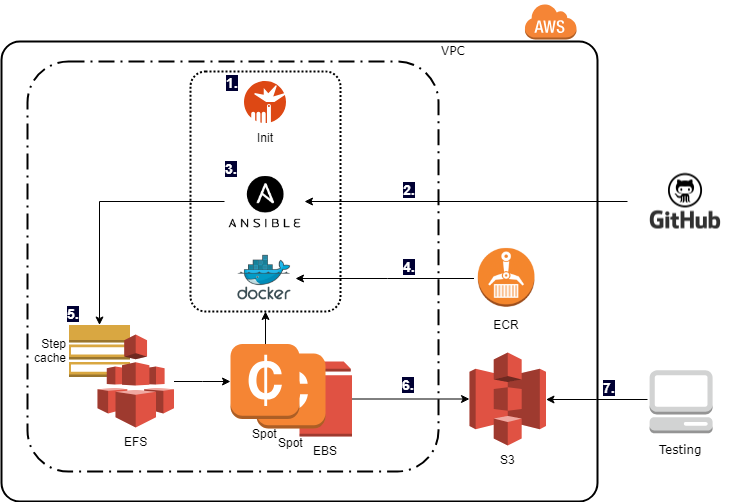
\includegraphics[width=.90\textwidth]{poc_zustand}
	\caption{Geodatenverarbeitung mit SPOT Instanzen.}
	\label{fig:ist_zustand}
\end{figure}

\subsection{Spot Flottenanfrage}
Als Setup für die Spot Flottenanfrage wurde ein sogenanntes Launch Template mit den wichtigsten Konfigurationen wie Sicherheitsgruppe, Wahl des AMI und User Data angelegt. Anschliessend wurde eine Spot Flottenanfrage basierend auf diesem Template erstellt. Wobei als Mindestanforderung an den Rechner 16 CPUs und 60 GB Memory waren. Als Option wurde gewählt, dass die Zielkapazität aufrechterhalten bleiben soll\footnote{Die Zielkapazität soll immer 1 sein.}: Somit wird nach jedem Interrupt automatisch eine neue Instanz mit der definierten Konfiguration zur Verfügung gestellt.

\subsection{Handling der Interrupts}
Wie im Kapitel \ref{kap:bugdet_instanzen} beschrieben, sind Spot Instanzen so günstig, weil sie einem jederzeit weggenommen werden können, um einem anderen Kunden zur Verfügung zu stellen. Also muss die Datenverarbeitung mit dem Handling von Interrupts umgehen können. 
Der Einfachheit halber hat der Autor gänzlich auf das \textit{Horchen eines bevorstehenden Interrupts} via RESTful Abfrage (In Anhang \ref{appendix:restful} beschrieben) oder \emph{CloudWatch} verzichtet und hat stattdessen die Datenverarbeitung als Serie betrachtet und in Schritte unterteilt. Sobald ein Schritt erledigt wird, wird dies auf dem EFS Volumen in einer Textdatei festgehalten. Falls es zu einem Interrupt kommen sollte, wird von der Spot Flotte die nächste Instanz bereitgestellt und die Publizierung macht bei dem Schritt weiter, der zuletzt in der Textdatei festgehalten wurde (Abbildung \ref{fig:ist_zustand}, Nr. 5).

\subsection{Die Datenverarbeitung als Code}
Mit der Entscheidung, die Spot Instanz via \emph{Cloud-Init}-Ansatz (Abb. \ref{fig:ist_zustand}, Nr. 1) mit Ansible zu Provisionieren\footnote{Und nicht mit einem neuen AMI.}, lag es auf der Hand, auch gleich dieselbe Technologie für die Realisierung der Datenverarbeitung zu verwenden (Nr. 3). 
Viele Annehmlichkeiten, wie die Nähe zur Shell und Python, das Logging und deklarativer Code zeigten sich in der Realisierung als hilfreich. Eines der ersten Kommandos welches das Initialisierungsskript ausführt, ist das klonen des Codes von github.com (Abb. \ref{fig:ist_zustand}, Nr. 2). Das Init-Skript wie auch das Ansible Playbook können auf \href{https://github.com/bfh-semesterarbeit/up-and-running-dataprocessing}{github.com/bfh-semesterarbeit} eingesehen werden.


\subsection{Testen der Datenstruktur}
Wie in Kapitel \ref{kap:sicherstellung_qualitaet} erwähnt, könnte die Datenverarbeitung bereits mit einfachen Bordmitteln vereinfacht werden. Es ist auch schon vorgekommen, dass die gelieferten Rohdaten selbst fehlerhaft waren. Da die alle gelieferten Rohdaten (KML und Collada) in XML geschrieben sind, wurde beschlossen einen kleinen Test mit grosser Wirkung in den automatischen Publikationsprozess mit einzubeziehen. Dieser Test macht nichts anderes, als die Dateien auf well-formed XML zu testen. 
Dieser Test schreibt den Namen aller fehlerhaften XML Dateien in eine Liste. Nach dem Testen wird die Länge dieser Liste überprüft und falls diese nicht leer ist, wird der gesamte Datenverarbeitung gestoppt. Diese Liste kann dann dem Auftraggeber zur Nachbearbeitung der fehlerhaften Daten ausgehändigt werden. Dieser Schritt passiert innerhalb Schritt Nr. 3 der  Abbildung \ref{fig:ist_zustand}.

\subsection{Datenverarbeitung}
Die eigentliche Datenverarbeitung, der Formatumbau\footnote{Rohdaten in das Web Format Cesium Tiles.}, wird mittels Docker Container ausgeführt. Um nicht von externen Services wie dockerhub.io abhängig zu sein und aus Neugier, wurde dafür ein AWS Container Repository\footnote{ECR} eingerichtet (Abbildung \ref{fig:ist_zustand}, Nr. 4.) \cite{9781484251003}. Das Kopieren der fertig verarbeiteten Webdaten auf S3 wird über die AWS CLI gemacht (Abb. \ref{fig:ist_zustand}, Nr. 6).

\subsection{Monitoring}
Bisher wird die Datenverarbeitung lediglich geloggt. Die verwendeten Tools\footnote{Der well-formed XML Test und der Output des Containers.} wie auch Ansible loggen in ein Verzeichnis im EFS, das gut zugänglich ist. Vor allem die Logdatei von Ansible ist ausführlich und macht eine Fehlersuche einfach.

Um die Last des Servers zu überprüfen, wurde lediglich die Standardüberwachung der Amazon Webconsole verwendet.

Bei einer allfälligen Integration des Prototypen in den Betrieb, müsste das Format und der Datenfluss dieser Logs an die Vorgaben der produktiven Infrastruktur angepasst werden.


\subsection{Inhaltliche Kontrolle der publizierten Daten}\label{kap:inhaltlich}
Um dem Datenlieferanten, dem Hersteller der 3D, zu ermöglichen, die 3D Daten inhaltlich zu prüfen, wurde ein sogenanntes codepen.io Projekt angelegt, dass auf den S3 Bucket des Prototypen zugreift und man so direkt die verarbeiteten 3D Gebäude inhaltlich überprüfen kann. Das Resultat, des Belastungstests (Kap. \ref{kap:belastungstest}), kann vorläufig\footnote{Bis am 1. November 2020} betrachtet und somit, zumindest theoretisch, inhaltlich überprüft werden. Es zeigt alle erfassten 3D Gebäude der Schweiz:
\href{https://codepen.io/rebert/pen/ExKZmmE}{codepen.io/rebert/pen/ExKZmmE}. Wobei zu erwähnen ist, dass nur die Gebäude vom S3 Testbucket der Prototypen kommen (Abb. \ref{fig:ist_zustand}, Nr. 7).

\subsection{Testen}
Da es sich um eine Datenverarbeitung und nicht um einen öffentlich zugänglichen Web Service handelt, wurde auf End-to-end Testing und Unit-Tests verzichtet. Es wurden lediglich Überprüft, ob die Datenverarbeitung auf den Spot Instanzen funktioniert. Hierzu wurden zwei Arten von Tests gemacht:

\subsubsection{Unerwartete Interrupts}
Da es in der ganzen Entwicklungsphase zu keinem einzigen Interrupt einer Spot Instanz gekommen ist, musste die Stabilität des Datenverarbeitungsprozesses auf unerwartete Interrupts manuell getestet werden. Um die Testphasen zu verkürzen, wurde die Menge der Eingangsdaten beschränkt\footnote{Auf ein Schweizerischer Kartenblatt 1:25'000.}.

Dieser Test wurde iterativ umgesetzt und der Code wurde bei Fehlern fortlaufend angepasst. 


\subsubsection{Belastungstest}\label{kap:belastungstest}
Der komplette Rohdatensatz, alle (erfassten) Gebäude der Schweiz, wurde verarbeitet. Dieser Test war sozusagen die Probe aufs Exempel. Bezüglich Anforderungen an die Rechnerleistung konnte auf Erfahrungswerte aufgebaut werden. Die Anforderungen an die Instanz mit dem gemounteten SSD Volumen haben gereicht. Dieser Test wurde auch dafür genutzt, den Output des Prototypen inhaltlich begutachten zu können, wie im vorhergehenden Kapitel (Kap. \ref{kap:inhaltlich} erwähnt. Aber auch die Erkenntnisse zur Wirtschaftlichkeit Kap. \ref{kap:wirtschaftlichkeit} wurden aus diesem Test abgeleitet.

